\label{Hoofdstuk 2}

\begin{sectionbox}{HandBrake geschiedenis}\end{sectionbox}
\ \\[6pt]
\subsection{Vorige versies}

Titer ontwikkelde HandBrake in 2003 en bleef de hoofdontwikkelaar tot april 2006. In dat jaar werd de offici"ele Subversion\index{Subversion} versie uitgebracht. Titer bleef nog actief op het HandBrake forum voor een korte periode totdat elk contact met hem verloren ging. Sinds mei-juni 2006 is er niemand in geslaagd om nog contact te leggen met titer. Sindsdien werden er ook geen offici"ele codeveranderingen meer gemaakt.

\subsection{MediaFork}

In September 2006 werkten Rodney Hester en Chris Long (elk afzonderlijk) om het H.264 video compressie formaat van Apple's IPod firmware\index{Firmware} (1.2) te extracten met behulp van reverse engineering\index{Reverse engineering}.Later ontmoetten ze elkaar op het HandBrake forum. Toevallig vulden ze elkaars werk aan met hun eigen bevindingen en begonnen ze samen te werken. Daardoor ontwikkelden ze een onstabiele maar compileerbare\index{Compileerbare} versie van HandBrake die het H.264 formaat ondersteunden. Hester en Long boekten aanzienlijk vooruitgang op gebied van stabiliteit, functionaliteit en GUI uiterlijk. Door de afwezigheid van titer was het onmogelijk om hun patch in te dienen in de HandBrake subversion opslagplaats.\\

Hun patch kon niet officieel ingediend worden als de nieuwe versie van HandBrake. Daarom cre"eerde Hester een subverion opslagplaats die de laatste HandBrake versie (0.7.1) spiegelde en startten ze met de verdere ontwikkeling hiervan. Hester en Long noemde dat nieuwe project MediaFork.

\subsection{2007 - heden}

Op 13 Februari 2007 werden Hester en Long gecontacteerd door titer die hen zijn volledige ondersteuning gaf en hen aanspoorde verder te gaan met de ontwikkeling. Er werden plannen gemaakt om MediaFork te integreren als de directe opvolger van HandBrake. De MediaFork website en forums werden verplaatst naar die van HandBrake en de volgende release van MediaFork werd officieel HandBrake genoemd.\\[24pt]

\begin{subsectionbox}{Features}\end{subsectionbox}
\subsubsection{Encoding}

Gebruikers hebben de mogelijkheid om de output aan te passen met bit rate, de maximum bestandsgrootte en sample rate via "constant quality".\\

HandBrake ondersteunt batch encoding\index{Encoding} door de Mac OS X, Linux en Windows grafische gebruikers interface (GUI) (zie figuren \ref{fig:Lgui},\ref{fig:Wgui} en \ref{fig:Igui}) en Command Line Interface (CLI). Third party scripts en UIs hebben precies dat doeleinde, zoals de HandBrake Batch Encoder en VideoScripts. Beide maken gebruik van een Command Line Interface om een wachtrij van verschillende bestanden in een enkele directory toe te staan.

\begin{figure}[!hp]
\centering
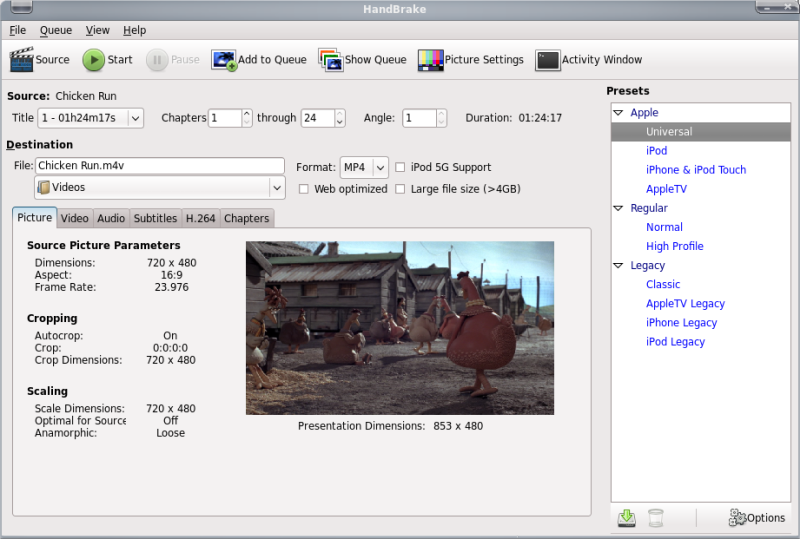
\includegraphics[width=0.5\textwidth]{linux1.png}
\caption{HandBrake GUI in Linux}
\label{fig:Lgui}
\end{figure}
\newpage
\begin{figure}[!hp]
\centering
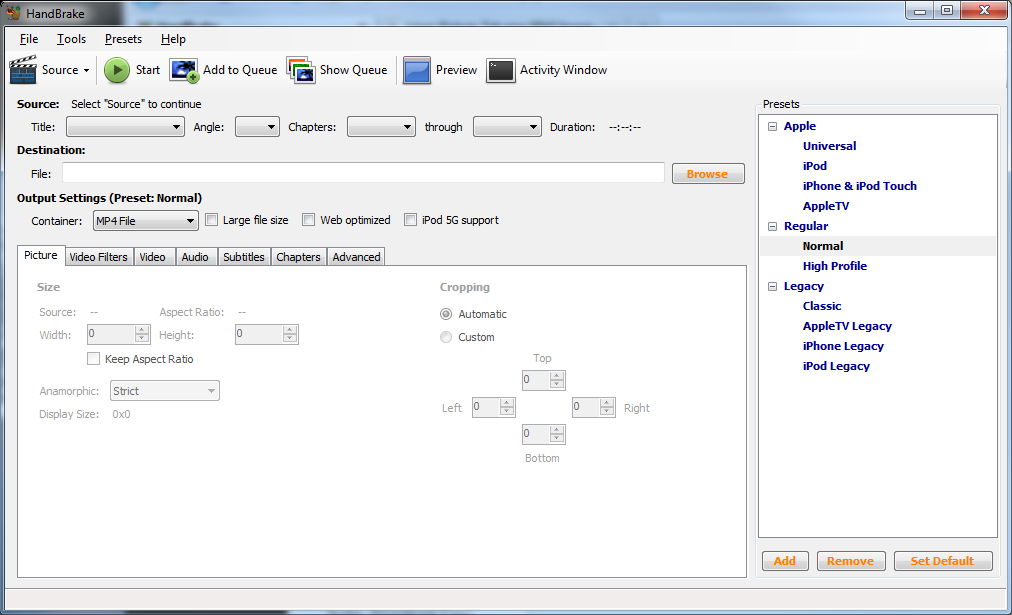
\includegraphics[width=0.75\textwidth]{win1.png}
\caption{HandBrake GUI in Windows}
\label{fig:Wgui}
\end{figure}
\begin{figure}[!h]
\centering
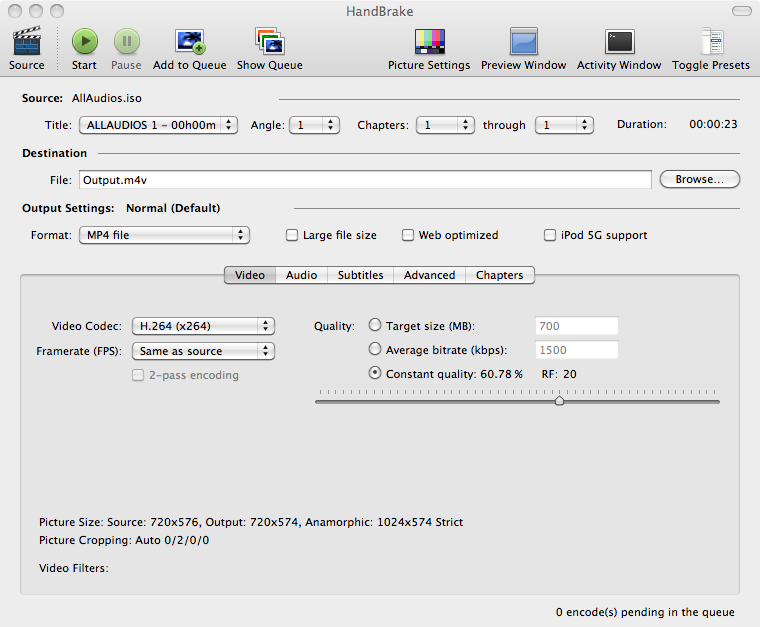
\includegraphics[width=0.75\textwidth]{mac1.png}
\caption{HandBrake GUI in IOS}
\label{fig:Igui}
\end{figure}
\newpage

\subsubsection{Video filtering}

HandBrake ondersteunt deinterlacing\index{Deinterlacing}, decombing\index{Decombing}, scaling\index{Scaling}, detelecine\index{Detelecine} and cropping\index{Cropping}.

\begin{list}{*}{}
\item Deinterlacing\cite{Deinterlacing}: is het proces van het converteren van interlaced video's, zoals vaak gebruikt in analoge televisiesignalen of 1080i formaat HDTV signalen, naar een niet-interlaced vorm. Een interlaced video frame bestaat uit twee gesynchroniseerde sub-velden, elk opeenvolgend gescand op even en oneven lijnen op de beeldsensor.

\item Decombing\cite{Decomb}: decombing maakt gebruik van deinterlancing. Deze past filter enkel toe op de frames die zichtbaar interlaced zijn, maar via decombing worden deze filter enkel toegepast waar nodig. De deinterlacing methode zou dat op alles toepassen en veroorzaakt onnodig kwaliteitsverlies.

\item Scaling\cite{scaling}: het verkleinen of vergroten van het beeld. Scaling is een niet-triviaal proces wat betreft een "trade-off" tussen effici"entie, smoothness en scherpte van het beeld.

\item Detelecine\cite{Telecine}: telecine is een proces voor het omzetten van fotografische film naar video. Het is het proces dat door bijna alle filmmaatschappijen gebruikt wordt om films naar DVD om te zetten, wanneer het origineel materiaal nog niet digitaal beschikbaar is.

\item Cropping\cite{Cropping}: refereert naar het verwijderen van stukken van het beeld voor het verbeteren van farming, accentueren van het werkelijke onderwerp en het veranderen van de aspect ratio. Dat wordt bijvoorbeeld veel gebruikt voor het verwijderen van (meestal Russische of Aziatische) ingeprogrammeerde ondertitels.
\end{list}

\subsubsection{Sources}

HandBrake, volgens hun website, converteert video's van zo goed als elk formaat naar een handvol moderne videoformaten en niet meer. Het breekt geen kopieprotecties. Een bepaalde vorm van input is DVD, afkomstig van een digitale opslagmedia zoals een video\_TS folder, een ISO image of direct van een CD-drive.

\paragraph{DVD}
\ \\[12pt]
HandBrake ontwikkelaars hebben de libdvdcss\cite{Libdvdcss} bibliotheek verwijderd van de applicatie in HandBrake versie 0.9.2. Het verwijderen van het Digital Rights Management (DRM)\cite{DRM} is mogelijk door VLC\cite{VLC} te installeren. Dat is een media speler waar de libdvdcss bibliotheek wel inbegrepen is.

\paragraph{Blu-ray Disk}  
\ \\[6pt]

Zoals bij DVD's ondersteunt HandBrake geen rechtstreekse decryptie voor Blu-ray Discs. HandBrake kan echter wel gebruikt worden om een Blu-ray Disc te transcoderen als de DRM vooraf verwijderd is door een third party application zoals bijvoorbeeld MakeMKV. MakeMKV is een populair programma, gemaakt voor het decrypten van Blu-ray Discs en wordt vaak gebruikt in combinatie met HandBrake.

\subsubsection{Support}

\begin{table}[!h]
\textbf{Input}\\
\centering
\begin{tabular}{ | l | l | l | }
\hline
Video\_TS & VOB & MPEG \\ \hline
MKV & AVI & BDAV MPEG\-2 \\ \hline
ISO image & MP4 & M2TS \\
\hline
\end{tabular}
\caption{Mogelijke input types in HandBrake}
\label{tab:input}
\end{table}

\begin{table}[!h]
\textbf{Output}\\
\centering
\begin{tabular}{ | l | l | l | l | }
\hline
\textbf{Container formats:} & MP4 & M4V & MKV \\ \hline
\textbf{Video formats:} & H.264 & MPEG-4 & Theora \\ \hline
\textbf{Audio formats:} & AAC & MP3 & AC-3 \\
\hline
\end{tabular}
\caption{Mogelijke output types in HandBrake}
\label{tab:output}
\end{table}

\pagebreak